%!TEX root = main.tex
\section{Methods\label{sec:methods}}
\subsection{Background and Motivation}
\par Visual query systems enable users to directly search for visualizations matching certain patterns through an intuitive specification interface. Early work in this space focused on interfaces to search for time series of interest, including TimeSearcher~\cite{Hochheiser2001,Hochheiser2004}, where the query is composed of one or more rectangular value-range selections, and QuerySketch~\cite{wattenberg2001sketching} and Google Correlate~\cite{mohebbi2011google}, where the query is sketched as a pattern. Subsequent work recognized the ambiguity of sketches and improved the expressiveness of sketched queries through finer specification interfaces and pattern-matching algorithms~\cite{ryall2005querylines,Holz2009}, as well as performed crowdsourced perceptual studies to understand how humans rank similarity in patterns subjectively~\cite{Eichmann2015,correll2016semantics,Mannino2018}. Table~\ref{table:relatedwork} summarizes the list of features offered by these existing systems.
% , including the use of soft constraints~\cite{ryall2005querylines} and implicit relaxed selection techniques~\cite{Holz2009}.
% In addition to this ongoing work, recent work have also performed crowdsourced perceptual studies to understand how humans rank similarity in patterns subjectively~\cite{Eichmann2015,correll2016semantics,Mannino2018}.
\begin{table} 
    % \begin{tabular}{@{} cl*{6}c @{}}
    %     % & & \multicolumn{6}{c}{Functionality Supported} \\[2ex]
    %     & & \hspace{-110pt}\rot{Pattern Specification} & \hspace{-110pt}\rot{Match Specification} & \hspace{-110pt}\rot{View Specification} & \hspace{-110pt}\rot{Slice-and-Dice}
    %     & \hspace{-110pt}\rot{Result Querying} &  \hspace{-110pt}\rot{Recommendation}\\
    %     \cmidrule{2-8}
    %     & Timesearcher \cite{Hochheiser2001,Hochheiser2004} &  &\OK   &\OK  &     &\OK  &   \\
    %     & QuerySketch \cite{wattenberg2001sketching} &\OK   &\OK  &  &   &    &   \\
    %     & QueryLines \cite{ryall2005querylines} &\OK   &\OK  &  &   &    &   \\
    %     & SoftSelect \cite{Holz2009} &\OK   &\OK  &  &   &    &   \\
    %     & Google Correlate \cite{mohebbi2011google} &\OK   &\OK  &  &   &    &   \\
    %     & TimeSketch \cite{Eichmann2015} &\OK   &\OK  &  &   &    &   \\
    %     & SketchQuery \cite{correll2016semantics} &\OK   &\OK  &  &   &\OK     &   \\
    %     & Qetch \cite{Mannino2018} &\OK   &\OK  &  &   &    &\OK    \\
    %     & Zenvisage (prototype) \cite{Siddiqui2017} &\OK   &\OK  &  &   &\OK     & \OK   \\
    %     & Zenvisage (after design study) &\OK   &\OK  & \OK  & \OK   &\OK     & \OK   \\
    %     \cmidrule[1pt]{2-8}
    % \end{tabular}
    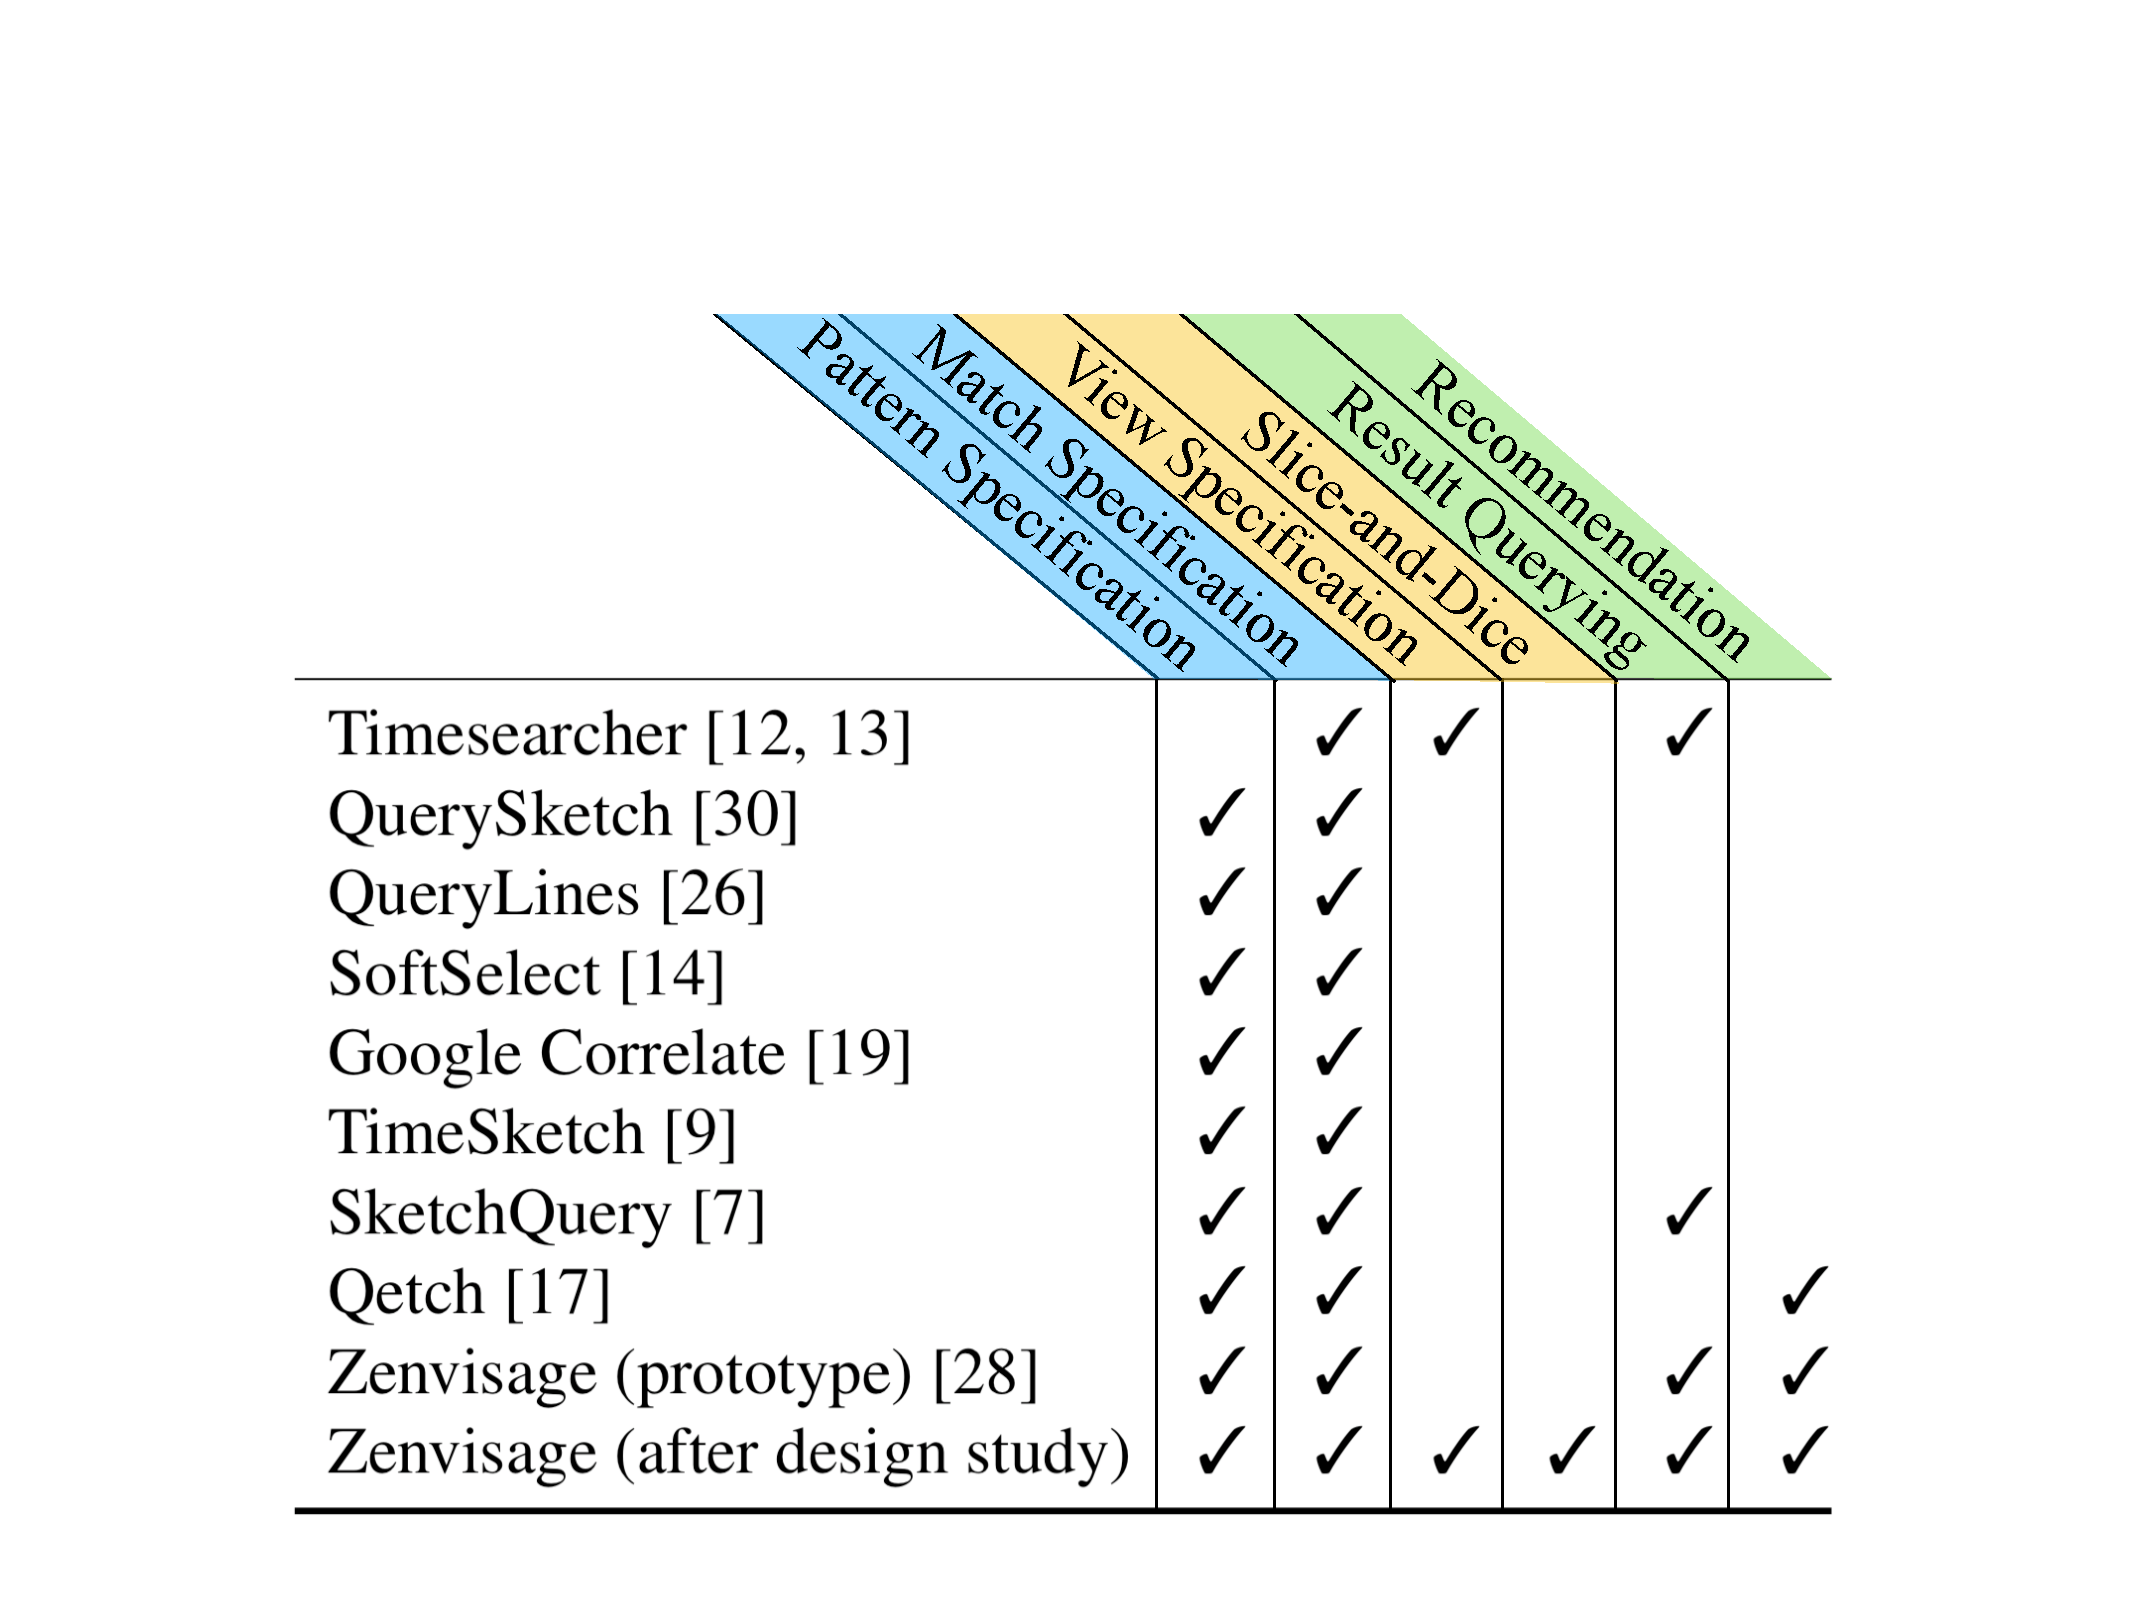
\includegraphics[width=0.75\linewidth]{figures/related_works_table.pdf}
    \caption{Table summarizing whether key functionalities of VQSs (columns) are covered by past systems (row), indicated by checked cells. Column header colors blue, orange, green represents three sensemaking process (top-down querying, search with context, and bottom-up querying) described in Section~\ref{sec:pd_findings}. The heavily-used, practical features in our study for context-creation and bottom-up inquiry is largely missing from prior VQSs.}
    \label{table:relatedwork}
    \vspace{-29pt}
\end{table}
\vspace{3pt}
\par While these systems have been shown to be effective for visual querying in controlled lab studies, they have not been evaluated in-situ on real-world use cases. In this work, we adopted a mixed methods research methodology that draws inspiration from ethnographic methods, iterative and participatory design, and controlled studies~\cite{Plaisant2004,lam2012empirical,shneiderman2006strategies,Muller1993} to more thoroughly understand the design space of VQSs and how various components of VQSs are used in practice. Participatory design has been successfully used in the development of interactive visualization systems in the past~\cite{Aragon2008,Chuang2012}. Sedlmair et al. \cite{Sedlmair2012} advocate that design study methodology is suitable for use cases in which the data is available for prototyping, but the task is only partially known and the information is partially in the user's head. %to understand how VQSs can be used in scientific data analysis. %In that regard, our scientific use cases with VQS is well-suited for a design study methodology, as we learn about the scientist's data and analysis requirements and design interactions that helps users translate their ``in-the-head'' specifications into actionable visual queries.
\subsection{Participatory Design}
\par  Working with researchers from three different scientific research groups, we identified the needs and challenges of scientific data analysis and potential opportunities for VQSs, via interviews and cognitive walkthroughs. We recruited participants by reaching out to research groups via email and word of mouth, who have experienced challenges in dealing with large amounts of data. We initially spoke to analysts from 12 different potential application areas and narrowed down to three use cases in astronomy, genetics, and material science for our participatory design study, based on their suitability for VQS as well as diversity in use cases. Six scientists from three research groups participated in the design of \zv. On average, participants had more than 8 years of research experience working in their respective fields. %\techreport{We list the participants in Table~\ref{participants}, and will refer to them by their anonymized ID as listed in the table throughout the paper.}
\par Given our early conversations with participants, we built a basic VQS to serve as the functional prototype in the design study. This early VQS prototype allowed users to sketch a pattern or drag-and-drop an existing visualization as a query, then the system would return visualizations that had the closest Euclidean distance from the queried pattern. The details of the system is described in \cite{Siddiqui2017,Siddiqui2017VLDB}, which focused on the system and scalability aspects of the VQSs.
	% \begin{figure}[ht!]
	% \centering
	% 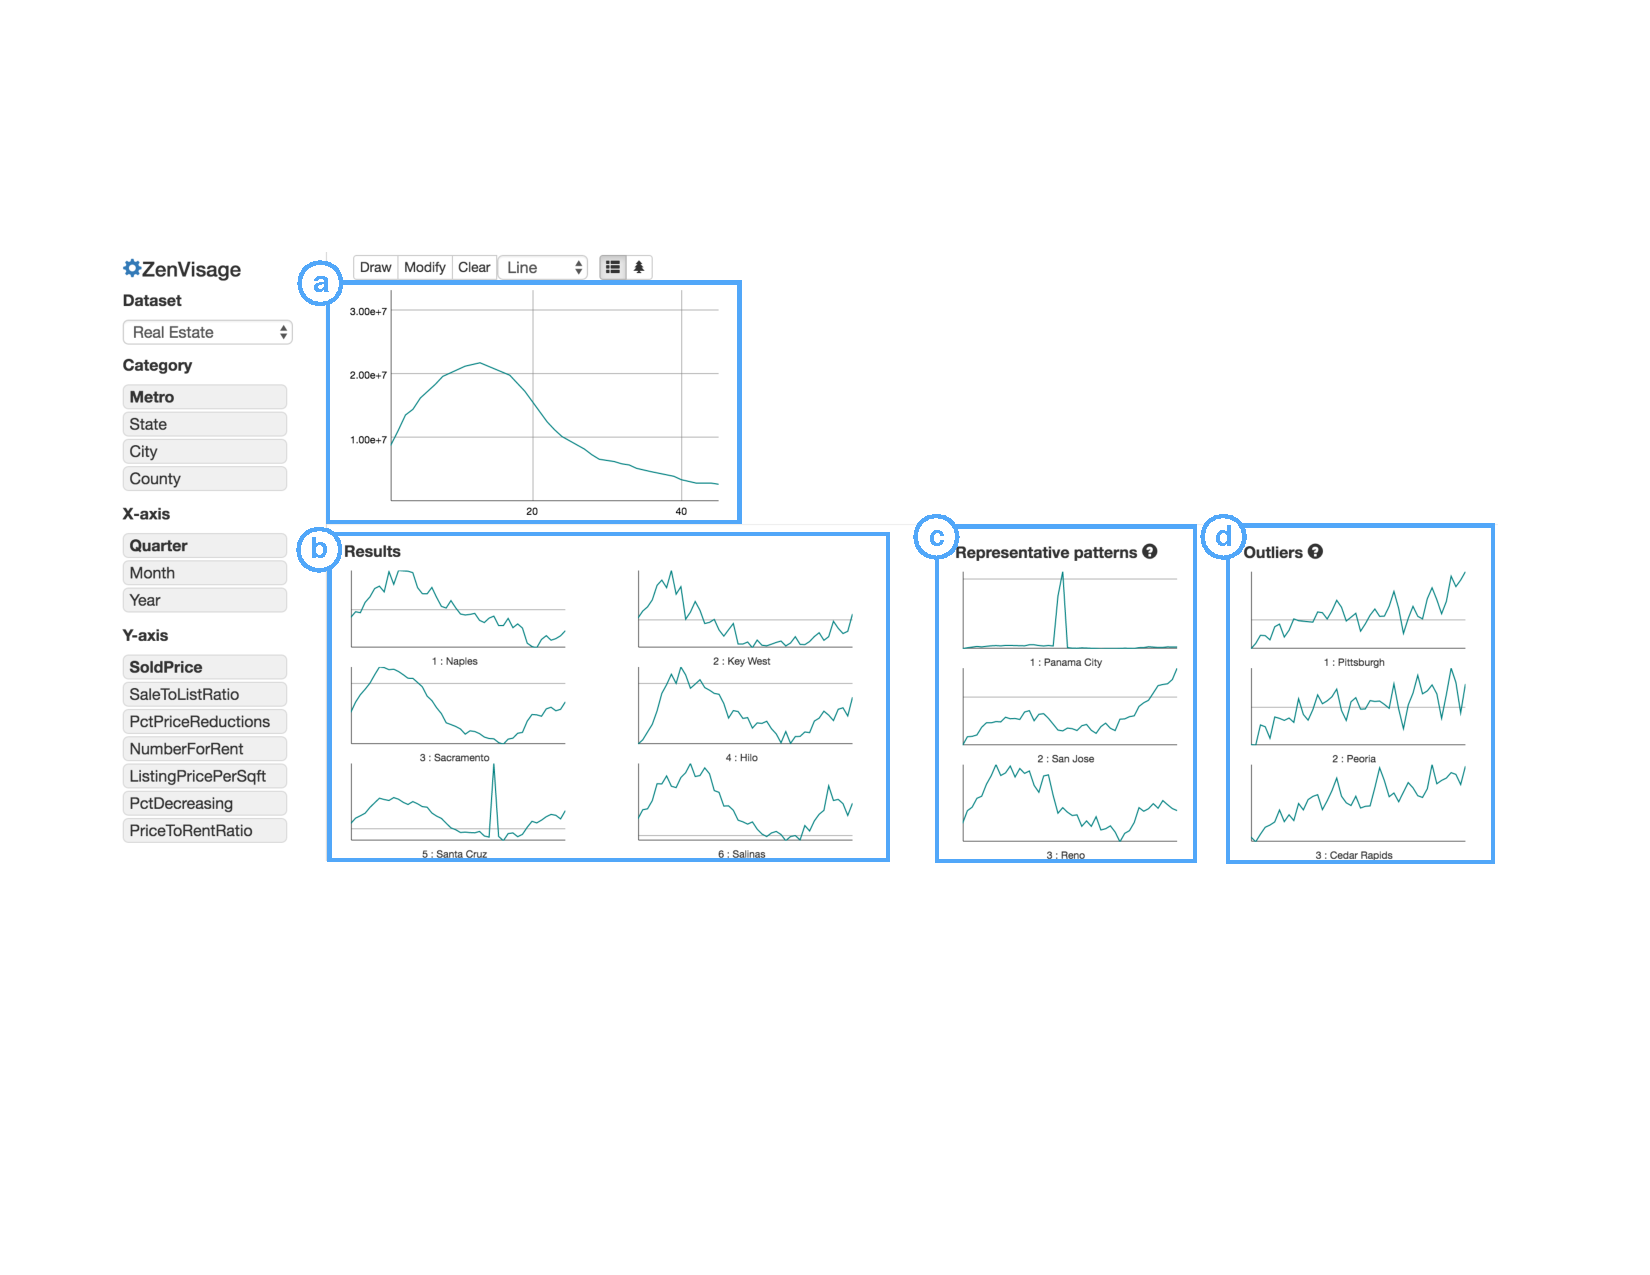
\includegraphics[width=\linewidth]{figures/oldZV_nozql.pdf}
	% \caption{The \zv prototype allowed users to sketch a pattern in (a), which would then return (b) results that had the closest Euclidean distance from the sketched pattern. The system also displays (c) representative patterns obtained through K-Means clustering and (d) outlier patterns to help the users gain an overview of the dataset.}
	% \label{oldZV}
	% \end{figure}
\par The use of functional prototypes is common and effective in participatory design to provide a starting point for the participants, as studied by Ciolfi et al.\cite{Ciolfi2016}. %For example, Ciolfi et al.\cite{Ciolfi2016} studied two different alternatives to co-design (starting with open brief versus functional prototype) in the development of museum guidance systems and found that while both approaches were equally fruitful, functional prototypes can make addressing a specific challenge more immediate and focused.
Our motivation for providing a functional prototype at the beginning of the participatory design sessions is to showcase capabilities of VQSs. Especially since VQSs are not common in the existing workflows of these scientists, participants may not be able to imagine their use cases without a starting point.
\par During the participatory design process, we collaborated with each of the teams closely with an average of two meetings per month, where we learned about their datasets, objectives, and how VQSs could help address their research questions. A summary timeline of our engagement with the participants and the features inspired by their use cases can be found in Figure \ref{timeline}. Participants provided datasets they were exploring from their domain, whereby they had a vested interest in using a VQS to address their own research questions. Through this process, we identified and incorporated more than 20 desired features into our VQS prototype, \zv, over the period of a year.
\begin{figure*}[!ht]
	\centering
	\captionsetup{justification=centering,margin=2cm}
	\vspace{-10pt}
	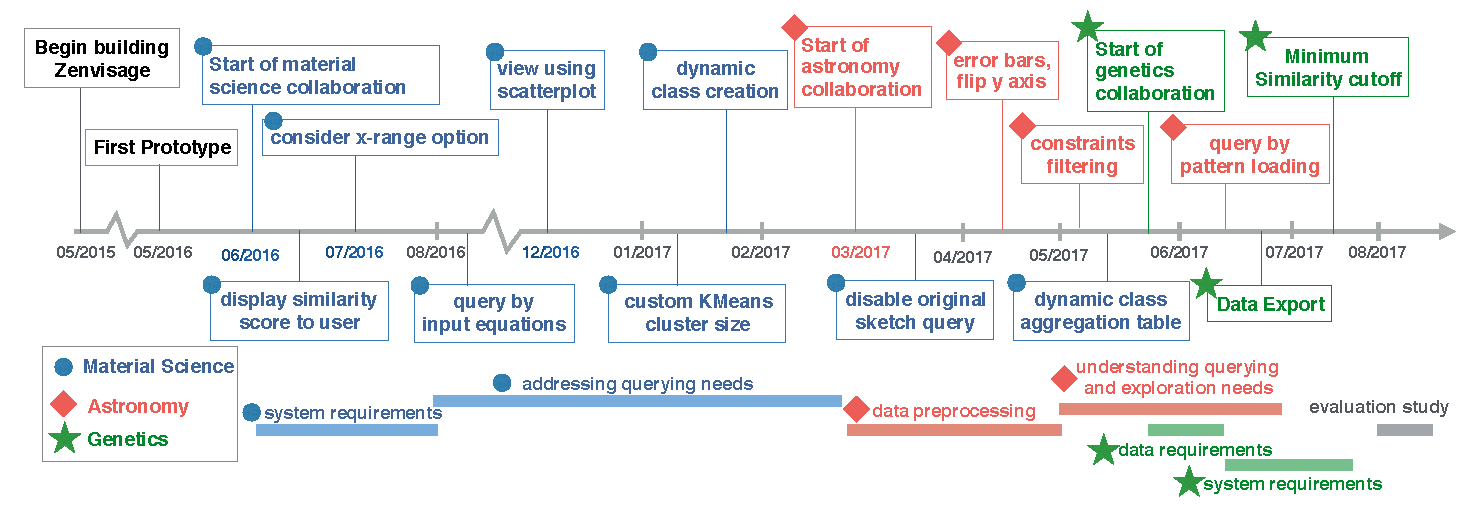
\includegraphics[width=6in]{figures/timeline_new.pdf}
	\vspace{-6pt}\caption{Participatory design timeline for the scientific use cases.}
	\label{timeline}
	\vspace{-10pt}
\end{figure*}
\subsection{Evaluation Study}
\par Visualization systems are often evaluated using controlled studies that measure the user's performance against an existing visualization baseline~\cite{Plaisant2004}. Techniques such as artificially inserting ``insights'' or setting predefined tasks for example datasets work well for objective tasks, \techreport{such as debugging data errors~\cite{kandel2011wrangler,Patel2010},} but they are unsuitable for trying to learn about the types of real-world queries users may want to pose on VQSs. %Due to the unrealistic nature of controlled studies, many have proposed using a more multi-faceted, ethnographic approach to understand how analysts perform visual data analysis and reasoning~\cite{Plaisant2004,lam2012empirical,shneiderman2006strategies,munzner2009nested,Sedlmair2012}.
In order to make the evaluation more realistic, at the end of our participatory design study, we opted for a qualitative evaluation where we invited participants to bring datasets that they have vested interests in to address unanswered research questions, in order to study how analysts interact with different VQS components in practice.
\par The evaluation study participants included the six scientists from participatory design, along with three additional ``blank-slate'' participants who had never encountered \zv before. While participatory design subjects actively provided feedback on \zv with their data, they only saw us demonstrating their requested features and explaining the system to them, rather than actively using the system on their own. So the evaluation study was the first time that all participants used \zv to explore their datasets.
\par Participants for the evaluation study were recruited from each of the three aforementioned research groups, as well as domain-specific mailing lists. Prior to the study, we asked the potential participants to fill out a pre-study survey to determine their eligibility. Eligibility criteria included: being an active researcher in the subject area with more than one year of research experience, and having worked on a research project involving data of the same nature as that used in the participatory design. Four of the evaluation studies were conducted remotely. Participants had the option of exploring their own dataset or an existing dataset that they provided to us during the participatory design process. All three blank-slate participants opted to explore their own datasets. %After loading their dataset, we emailed them a screenshot of a visualization from our tool to verify that we configured the system to meet their needs.
\par At the start, participants were provided with an interactive walk-through explaining the system details and given approximately ten minutes to experience a guided exploration of our VQS with a preloaded real-estate example dataset from Zillow \cite{zillow}.\techreport{This dataset contained housing data for various cities, metropolitan areas, and states in the U.S. from 2004-15.} After familiarizing themselves with the tool, we loaded the participant's dataset and encouraged them to talk-aloud or use external tools as needed during the data exploration phase.% and suggested an appropriate choice of axis to begin the exploration.
%\par During the exploration phase, participants were informed that they could use other tools as needed.
If the participant was out of ideas\ccut{ for three minutes}, we suggested one of the ten main functionalities in \zv \techreport{\footnote{query by sketching, drag-and-drop, pattern loading, input equations, representative and outliers, narrow/ignore x-range options, filtering, data smoothing, creating dynamic classes,  data export}}that they had not yet used. If any of these operations were not applicable to their specific dataset, they were allowed to skip the operation after having considered how it may or may not be applicable to their workflow. The user study ended after they covered all ten main functionalities. On average, the main exploration phase lasted for 63 minutes. After the study, we asked them open-ended questions about their experience.
